\documentclass[a4paper,11pt]{article}
\usepackage[utf8]{inputenc}
\usepackage[spanish]{babel}
\usepackage{amsmath, amssymb}
\usepackage{graphicx}
\usepackage{float}
\usepackage{url}
\usepackage{geometry}
\usepackage{titlesec}
\usepackage{hyperref}
\geometry{margin=2.5cm}
\setlength{\parskip}{0.8em}
\setlength{\parindent}{0pt}
\titleformat{\section}{\Large\bfseries}{\thesection}{1em}{}

\title{\textbf{Implementación desde cero de un Motor de Redes Neuronales}}
\author{Raúl Mendoza \and Adrián Ojeda \and Jesus Varela}
\date{Optimización y Heurística \\ Escuela de Ingeniería Informática \\ Universidad de Las Palmas de Gran Canaria}

\begin{document}

\maketitle

\begin{abstract}
Este trabajo presenta la implementación desde cero de un motor de redes neuronales densas (Fully Connected Neural Network) utilizando exclusivamente \texttt{NumPy} y \texttt{matplotlib}, sin recurrir a librerías de aprendizaje profundo como TensorFlow o PyTorch. 
El sistema permite definir arquitecturas con número variable de capas y neuronas, entrenar mediante el algoritmo de \textit{backpropagation} y optimizar los parámetros con \textit{Adam}. 
Los experimentos realizados sobre los conjuntos XOR e IRIS demuestran un aprendizaje efectivo, alcanzando una precisión del 91.3\% en la clasificación multiclase de IRIS. 
La correcta convergencia de las curvas de pérdida confirma la validez del motor desarrollado.
\end{abstract}

\section{Introducción}
Las redes neuronales artificiales constituyen uno de los pilares fundamentales del aprendizaje automático. 
Su capacidad para modelar relaciones no lineales complejas las convierte en una herramienta esencial para la resolución de problemas de clasificación y regresión.
El objetivo de este proyecto es desarrollar, desde un enfoque pedagógico, un \textbf{motor de redes neuronales densas totalmente funcional}, implementando manualmente los cálculos de propagación directa, retropropagación y actualización de parámetros.

El proyecto forma parte de la asignatura \textit{Optimización y Heurística} del Grado en Ciencia e Ingeniería de Datos y se ajusta a los requisitos mínimos definidos en la guía de la primera entrega. 

\section{Métodos y Conjuntos de Datos}

\subsection{Arquitectura de la red}
El motor permite definir redes de tipo \textit{Feedforward Neural Network} con un número configurable de capas y neuronas. 
Cada capa está compuesta por pesos \(W\), sesgos \(b\) y una función de activación. 
La salida de cada capa se calcula como:
\[
z^{(l)} = W^{(l)}a^{(l-1)} + b^{(l)}, \quad a^{(l)} = f(z^{(l)})
\]
donde \(f\) puede ser \textit{sigmoid}, \textit{tanh}, \textit{ReLU} o \textit{softmax}.

\subsection{Backpropagation}
El algoritmo de retropropagación se implementó manualmente aplicando la regla de la cadena. 
El gradiente de la función de pérdida respecto a los pesos y sesgos se calcula de la forma:
\[
\frac{\partial L}{\partial W^{(l)}} = \delta^{(l)} (a^{(l-1)})^T, \quad 
\frac{\partial L}{\partial b^{(l)}} = \delta^{(l)}
\]
donde \(\delta^{(l)}\) representa el error propagado hacia atrás.

\subsection{Función de pérdida y optimización}
Se implementaron las funciones de pérdida \textit{MSE} y \textit{Cross-Entropy}. 
Para la optimización se desarrolló el algoritmo \textit{Adam}, que combina las ventajas de los métodos de momento e \textit{RMSProp}, ajustando la tasa de aprendizaje de cada parámetro en función de su historial de gradientes.

\subsection{Conjuntos de datos utilizados}
Se realizaron dos experimentos principales:
\begin{itemize}
    \item \textbf{XOR:} problema clásico no lineal de dos entradas y dos salidas, utilizado para verificar la correcta implementación del \textit{forward} y \textit{backpropagation}.
    \item \textbf{IRIS:} conjunto de datos de clasificación multiclase con 150 muestras, 4 características y 3 clases (\textit{setosa}, \textit{versicolor}, \textit{virginica}). Los datos se normalizaron y se aplicó \textit{one-hot encoding} a las etiquetas.
\end{itemize}

\section{Detalles de Implementación}

El código se estructura modularmente en un paquete \texttt{src/} con las siguientes clases principales:
\begin{itemize}
    \item \texttt{Dense:} representa una capa completamente conectada con su activación.
    \item \texttt{NeuralNetwork:} gestiona las capas, el cálculo de gradientes y la inferencia.
    \item \texttt{Adam:} implementa el optimizador adaptativo.
    \item \texttt{Trainer:} controla el ciclo de entrenamiento, generación de mini-batches, cálculo de pérdidas y validación.
\end{itemize}

El entrenamiento se realiza por mini-lotes de tamaño variable y permite fijar una semilla aleatoria para garantizar la reproducibilidad.

\section{Experimentos y Resultados}

\subsection{Experimento 1: XOR}
Para el conjunto XOR, se empleó una red 2--4--2 con activaciones \textit{tanh} y \textit{softmax}. 
La pérdida convergió a valores próximos a cero en menos de 100 épocas, clasificando correctamente los cuatro patrones de entrada. 
Este resultado valida la implementación básica del motor.

\subsection{Experimento 2: IRIS}
En el caso de IRIS, se utilizó una red 4--16--3, activación \textit{ReLU} en la capa oculta y \textit{softmax} en la salida, con pérdida \textit{cross-entropy} y optimizador Adam (\(lr=0.01\)). 
Tras 120 épocas de entrenamiento, se obtuvo una pérdida final de \(L_{val} \approx 0.05\) y una \textbf{precisión en test del 91.3\%}. 
La Figura~\ref{fig:curva_loss} muestra la evolución de las pérdidas de entrenamiento y validación.

\begin{figure}[H]
    \centering
    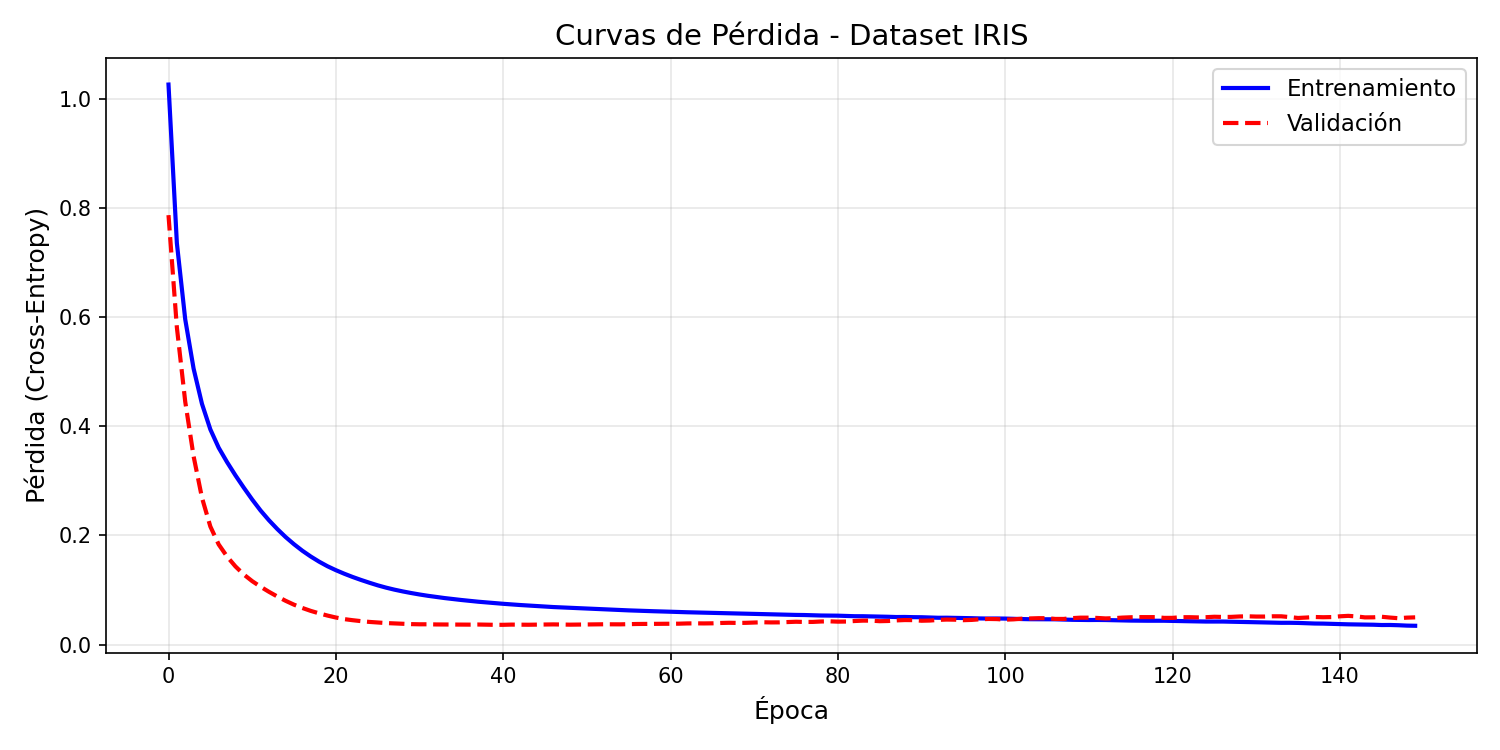
\includegraphics[width=0.7\textwidth]{fig_loss_iris.png}
    \caption{Curva de pérdida del entrenamiento sobre IRIS.}
    \label{fig:curva_loss}
\end{figure}

La matriz de confusión obtenida fue:
\[
\begin{bmatrix}
10 & 1 & 0 \\
0 & 4 & 1 \\
0 & 0 & 7
\end{bmatrix}
\]
Mostrando una confusión leve entre las clases \textit{versicolor} y \textit{virginica}, algo esperable dada su proximidad en el espacio de características.

\section{Conclusiones y Trabajo Futuro}
El motor desarrollado cumple con todos los requisitos mínimos establecidos en la práctica:
\begin{itemize}
    \item Implementación modular y reproducible.
    \item Backpropagation y optimización Adam correctos.
    \item Entrenamiento con mini-batches y división train/val/test.
    \item Pruebas exitosas en XOR e IRIS.
\end{itemize}

Como trabajo futuro, se propone:
\begin{itemize}
    \item Añadir nuevas funciones de activación (\textit{LeakyReLU}, \textit{ELU}).
    \item Implementar regularización L2 y \textit{dropout}.
    \item Incluir otros optimizadores como \textit{SGD+Momentum} y \textit{RMSProp}.
    \item Ampliar los experimentos a datasets más complejos como MNIST.
\end{itemize}

\section{Bibliografía}
\begin{itemize}
    \item S. Haykin, \textit{Neural Networks and Learning Machines}, 3rd ed., Pearson, 2008.
    \item I. Goodfellow, Y. Bengio, A. Courville, \textit{Deep Learning}, MIT Press, 2016.
    \item Documentación oficial del dataset IRIS: \url{https://archive.ics.uci.edu/ml/datasets/iris}.
\end{itemize}

\end{document}
